\documentclass[14pt, a4paper]{extarticle}

%\usepackage[T2A]{fontenc}
\usepackage[utf8]{inputenc} 
\usepackage[english,russian]{babel}
\usepackage{ upgreek }
\usepackage{url}
%\usepackage{pscyr}

%\renewcommand{\rmdefault}{ftm}
\usepackage{setspace}
\onehalfspacing

\usepackage{changepage}
\usepackage{indentfirst} %первый абзац
\usepackage[noend]{algorithmic}
\usepackage{amssymb, amsmath, multicol,amsthm}
\usepackage{tabularx}
\usepackage{enumitem, multicol}
\usepackage{titleps,lipsum}
\usepackage{mathrsfs}
\usepackage{verbatim}
\usepackage{pb-diagram}
\usepackage{graphicx}
\graphicspath{ {images/} }
\usepackage{wrapfig}
\usepackage{xcolor}
\definecolor{new}{RGB}{255,184,92}
\definecolor{news}{RGB}{112,112,112}
\usepackage{wallpaper}
\usepackage{float}
\usepackage{hyperref}
\usepackage{multirow}
\usepackage{longtable}
\usepackage{rotating} 
\usepackage{epsfig}
\usepackage{subfig}
\hypersetup{
	linkbordercolor=new,
}


\allowdisplaybreaks
%\usepackage{geometry}
%\geometry{top=3cm,bottom=2cm,left=2cm,right=2cm}

\usepackage[margin=2cm,left=3cm,right=1.5cm]{geometry}


\binoppenalty=5000
\parindent=1cm

\renewcommand{\div}{\operatorname{div}}
\newcommand{\grad}{\operatorname{grad}}
\newcommand{\rot}{\operatorname{rot}}
\newcommand{\const}{\operatorname{const}}
\newcommand{\diag}{\operatorname{diag}}
\renewcommand{\leq}{\leqslant}
\renewcommand{\geq}{\geqslant}
\newtheorem{Lemma}{Лемма}
\def\proofname{Доказательство}


\begin{document}
	
	\vskip 3mm
	
	\setcounter{page}{1}
	%%%%%%%% титульный лист %%%%%%%%%%%%%%%%%%%%%%%%%%%%%%%%%
	\begin{center}
		\thispagestyle{empty}
		
		{ Министерство общего и профессионального образования \\}
		{ Российской Федерации \\}
		
		
		{ Московский Физико-технический институт \\}
		
		{(Государственный университет) \\}
		
		{ Факультет управления и прикладной математики \\}
		
		{ Кафедра Acronis \\[4cm]}
		
		{ \bf \Large Выпускная квалификационная работа\\}
		
		{ \bf \Large{"Anomaly detection"\\[1cm]} }
		
		{\bf {Студента 4-го курса Лемихова Александра Алексеевича}\\[3cm]}
		
	\end{center}
	
	\begin{flushright}
		\bf{Научный руководитель}\\
		\bf{Андрей Кулага}\\[4cm]
	\end{flushright}
	
	\begin{center}
		Москва, 2020
	\end{center}
	
	\newpage
	\tableofcontents
	\newpage
	
	
	\section{Аннотация}
	\sectionmark{Аннотация}
	В данная выпускная квалификационная работа посвящена предсказанию временных рядов. 
	Основной упор сделан на распространении одного метода на всё многообразие дата центров компании Acronis. 
	Результатом работы является метод предоработки входных данных, построений предсказаний и оценки результатов которые подходят для существенной части хранилищ.
	
	\section{Введение}
	\sectionmark{Введение}
	Данная работа является вспомогательным инструментом для системы автоматического определения аномалий.
	Множество методов определения аномалий используют предсказания временных рядов. 
	Ошибка в предсказаниях является нарушением установленных связей в системе и может пролить свет на неточности системы, которые невозможно уловить человеческими усилиями, ввиду огромного количества данных.
	
	Для автоматизации обработки данных предлагается использовать базовые механизмы машинного обучения - линейную регрессию. 
	Её преимуществом является интерпретируемость, возможность на каждом шаге отследить корректность модели.
	
	На сегодняшний день построение предсказательных систем является важной областью машинного обучения.
	Разработано множество подходов к предсказанию временных рядов множества переменных.
	Несмотря на это, поиски литературы об универсальности методов для различных систем не принесли результатов. 
		
	Основной целью работы является выделение из класса моделе \texttt{SARMA} той, которая будет одинаково хорошо подходить под кажый instance продукта ABGW Acronis.
	
	Работа разделена на следующие части:
	\begin{itemize}
	\item Обзор методов, которые могут быть применены в данной задаче
		\begin{itemize}
		\item Сбор данных
		\item Предобработка
		\item Модель
		\item Оценка модели
		\end{itemize}
	\item Далее каждый этап модели представлен в отдельной секции более подробно
	\end{itemize}
	
	В процессе работы был исследован класс моделей \texttt{ARMA} и предложено универсальное решение, подходящее под большое множество инстансов.
				
	\section{Постановка задачи}

	Цель задачи - приспособить широко известный концепт - линейную регрссию для предсказания и исследования временных рядов.
	Как основной концепт, исопльзуемый для построения модели в работе используется касс моделей \texttt{ARMA}.
	
	Идея исследовать линейные зависимости в системе давно развивается Андереем Кулагой и его студентами.
	Важное свойство - линейность, была обнаружена зорким глазом, при наблюдении метрик системы в Graphana. 
	Линеные взаимосвязи был выявлены среди признаков, со следующей сутью:
	\begin{itemize}
	\item Производная суммарной задержки iop операций.
	\item Производная суммарного счётчика запросов, вызвавших задержку.
	\item Число подключений.
	\item Производная суммарной задержки, видной польователю.
	\end{itemize}
	
	На сегодняшний день Acronis собирает данные о много большем числе признаков системы.
	Из этого возникает возможность исследования большего числа метрик, для построения более качественной модели.
	
	Ниже перечислены возможные подхды, которые были применены к системе
	
	
	\section{Подходы к решению}
	\subsection{Сбор данных}
	Для построения системы, строящей предсказания на основе взаимосвязи между метриками необходима система сбора и хранения данных. 
	В компании Acronis для этого используется Prometheus \cite{lib_prometheus}, предоставляющий возможность выгрузки данных с дискретность не выше 1 минуты.
	 Как оказалось, этого вполне хватает для успешного построения модели.
	Сбор данных продолжается исследованием структуры данных.
	
			
	\subsection{Выбор данных}
	Acronis использует сервис мониторинга Prometheus, с помощью которого можно загрузить данные в удобном формате. 
	В работе выводы построены на данных в период с 14/01/2020 00:01 до 01/05/2020 00:01 со следующих дата-центров:
	\begin{enumerate}
		\item au2-acs1
		\item us6-acs2
		\item eu3-acs1
		\item us3
	\end{enumerate}
	Необходимо выбрать ограниченный набор дата-центров, чтобы трудоёмкость вычислений и объёмы данных не мешали построению выводов. 
	Тем не менее этот набор данных позволяет наблюдать различные нагрузки и шаблоны поведения системы.
	
	В качестве целевой метрики, метрики для предсказаний была выбрана следующая метрика:
	\begin{equation}
		 \texttt{abgw\_iop\_latency\_ms\_sum\{err="OK", proxied="0", iop="isync"\}}\label{target_metric}
	 \end{equation}
	 Исследуя все остальные метрики был составлен набор информативных метрик.
	 Популярные примеры не информативны метрик - константы на довольно длинных участках. 
	 
	 Кроме того, следует упомянуть, что запрос принципиально возвращает матрицу.
	 Например \texttt{abgw\_client\_conns\_cur\{dc="us3", instance="5"\}} вернёт матрицу, всех возможных \texttt{abgw\_client\_conns\_cur} для заданого инстанса по различным фильтрам. 
	 Одним из таких фильтров является \texttt{proto="v1"}, который возник неожиданно и не на всех инстансах.
	 Было принято решение перейти от матрицы к вектору - метрике путём суммирования построчно. Такое решение не изменит сути признаков и их интерпритация не изменится.
	 
	Список рассматриваемых метрик приведён ниже:
	 \begin{enumerate}
	 	\item \texttt{abgw\_iop\_latency\_ms\_count\{err="OK"}, \\
	 	\texttt{job="abgw"}, \texttt{iop="isync"}, \texttt{proxied="0"\}}
	 	\item \texttt{abgw\_account\_lookup\_errs\_total\{err="OK"\}}
	 	\item \texttt{abgw\_account\_pull\_errs\_total\{err="OK"\}}
	 	\item \texttt{abgw\_accounts}
	 	\item \texttt{abgw\_append\_throttle\_delay\_ms\_total}
	 	\item \texttt{abgw\_client\_conns\_cur}
	 	\item \texttt{abgw\_client\_conns\_total}
	 	\item \texttt{abgw\_fds)}
	 	\item \texttt{abgw\_file\_lookup\_errs\_total\{err="OK"\}}
	 	\item \texttt{abgw\_files}
	 	\item \texttt{abgw\_read\_bufs}
	 	\item \texttt{abgw\_read\_bufs\_bytes}	
	 	\item \texttt{abgw\_read\_bytes\_total\{proxied="0"\}}
	 	\item \texttt{abgw\_read\_reqs\_total}
	 	\item \texttt{abgw\_req\_latency\_ms\_count}
	 	\item \texttt{abgw\_req\_latency\_ms\_sum}
	 	\item \texttt{abgw\_account\_lookup\_errs\_total}
	 	\item \texttt{(abgw\_account\_pull\_errs\_total\{err="OK"\}}
	 \end{enumerate}\label{list_of_metrics}


	\subsection{Предобработка}
	Теория временных рядов предполагает разложение ряда на трендовую и сезонную составляющие, обуславливаемые наблюдаемыми признаками. 
	Помимо них присутствует ошибка, которая в идеальном случае должна быть нормальной центрированной случайной величиной.
	И последняя составляющая - циклы, отличающиеся от сезонности непостоянностью периода.
	
	Кроме стационарности важно распределние, соответсвующее потоку данных.
	Особенности в данных, такие как выбросы и пропуски должны быть вявлены и процесс вся модель, вместе с предобработкой должна учитывать их.

	Задача предобработки - получить стационарные данные, удовлетворяющие этим требованиям.


	\subsection{Модель}

	Имея набор данных - метрик нужно сформировать признаковое пространство и гипотезу об ошибке.
	Максимизация функции правдоподобия для выбранной вероятностной модели приводит к выбору функции потерь.
	Как правило, такой поход требует дополнения в виде регуляризаторов - штрафа за сложность и нестабильность модели или же изменения гипотезы о вероятности ошибки.
	
	Построение универсальной модели для семейства объектов предполагает подбор гиперпараметров - параметров, которые подбираются один раз на некоторое множество моделей.
	Такие параметры присутствуют, как правило, в большинстве алгоритмов.	
	Для подбора гиперпараметра функция ошибки должна быть масштабируемой - корректно оценивать качество модели, например, не зависимо от нагрузки, количества пользователей.


	\subsection{Оценка модели}
	В рамках исследования класса моделей \texttt{ARMA} можно выделить следующие критерия качества модели:
	\begin{itemize}
	\item Гетероскедастичность
	\item Однородность временного ряда ошибки
	\item Центрированность ошибки
	\end{itemize}
	
	Общепринятный проверки качества - анализ графиков.
	Также можно проверять статистические гипотезы.
	Однако, модель применена к огромному количесвту данных и поэтому мощность критериев становится слишком велика \cite{lib_large_samples}.
	
	
	\section{Предобработка}
	\sectionmark{Предобработка}
	\subsection{Тренд}
	
	\begin{figure}[h]
		\centerline{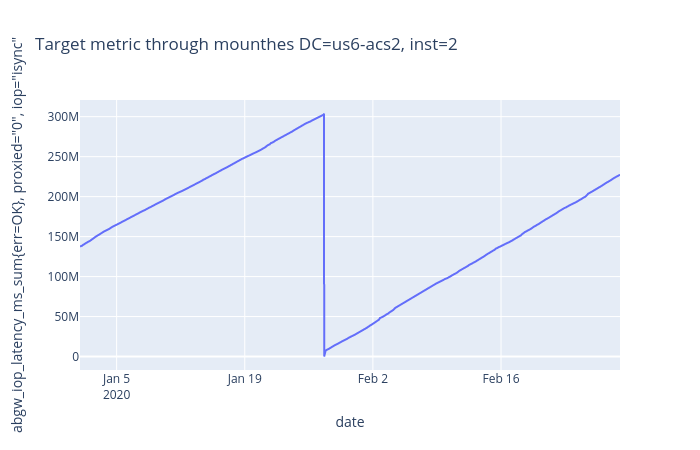
\epsfig{file=Figures/target_metric_1.png, scale=0.5}} 
		\caption{Целевая метрика \ref{target_metric} за исследуемый период}
		\label{target_metric_fig1}
	\end{figure} 
	
	На рис.\ref{target_metric_fig1} показан график целевой переменной. 
	Уменьшение целевой переменной между 19 марта и 2 февраля - явный признак перезагрузки системы. 
	Такие участки необходимо удалить из данных для построения зависимостей.
	Кроме того в данных явно присутствует тренд. 
	Самый простой способ избавиться от тренда - перейти к приращениям, производной. 
	Такой подход оказался достаточно универсальным.  
	\begin{figure}[!htb]
		\minipage{0.49\textwidth}
		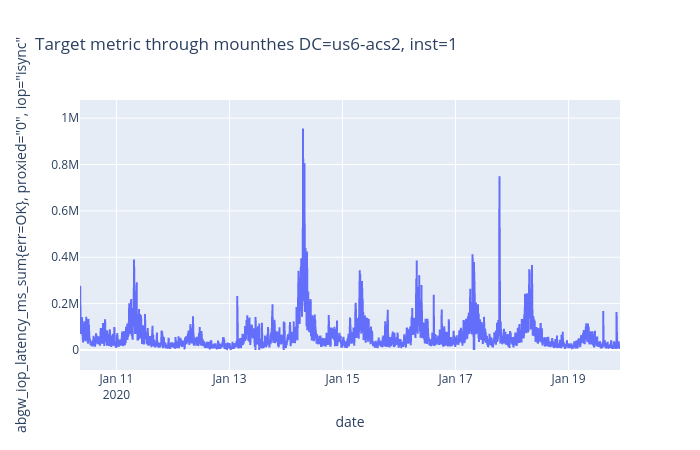
\includegraphics[width=\linewidth]{Figures/target_der_1.png}
		\caption{Целевая метрика в пространстве производных, dc=us6-acs2, inst=23}\label{fig:target_der_fig1}
		\endminipage\hfill
		\minipage{0.49\textwidth}
		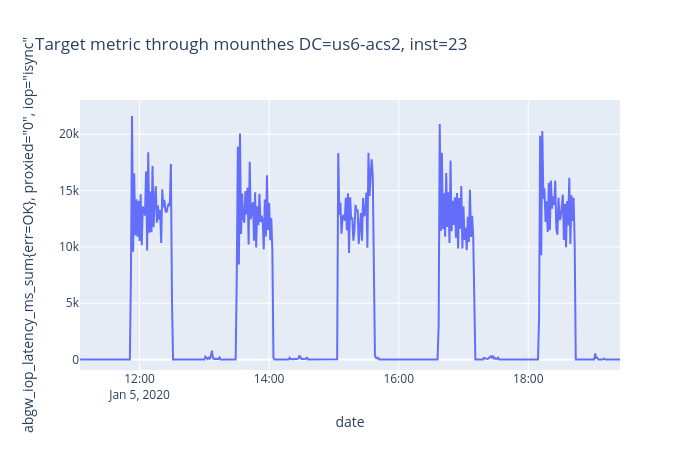
\includegraphics[width=\linewidth]{Figures/target_der_2.png}
		\caption{Целевая метрика в пространстве производных, dc=us6-acs2, inst=1}\label{fig:target_der_fig2}
		\endminipage
	\end{figure}

	Результатом дифференцирования суммарной задержки является накопленная за минут задержка. Её можно интерпретировать как загрузку системы.
	
	\subsection{Масштабирование}
	В отсутствии тренда метрика локализована на компакте. Однако стоит отметить разницу загрузки систем в десятки раз.	
	Один из способов избавиться от такой разнице в загрузке - перейти к масштабированным переменным на $[0;1]$. Такой переход продемонстрирована в формуле \ref{MinMax_sc}.
	
	\begin{equation}
		x_{sc} = \frac{x - min(x)}{max(x) - min(x)} \label{MinMax_sc}
	\end{equation}
	Применение такого масштабирования обеспечит простую интерпретацию целевой переменной - доля максимальной загрузки.
	
	Однин из минусов такой предобработки - неустойчивость к выбросам.
	Стоит упомянутб преобразование, не страдающее таким неугом - преобразование Yeo-Johnson:
	
	\begin{align}
	\hat{x}_{\lambda} = 
	\begin{cases}
	((x+1)^{\lambda }-1)/\lambda &{\text{if }}\lambda \neq 0,x\geq 0\\
	\log(x+1)&{\text{if }}\lambda =0,x\geq 0\\
	-[(-x+1)^{(2-\lambda )}-1]/(2-\lambda )&{\text{if }}\lambda \neq 2,x<0\\
	-\log(-x+1)&{\text{if }}\lambda =2,x<0
	\end{cases} \label{Yeo-Joh}
	\end{align}
	
	Парметр $\lambda$ выбирается, чтобы приблизить распределение признака к нормальному.
	Сравнение этих двух подходов представлено в \cite{lib_sklearn_transformer_outliers}.
	Для построения можели, в первом приближении, в работе используется \texttt{MinMaxScaler} (\ref{MinMax_sc}).
	
	
	
	\subsection{Сезонность}
	На рис.\ref{fig:target_der_fig1} и рис.\ref{fig:target_der_fig2} легко видеть сезонность.
	В этой части приведено рассмотрение несколько способов предобработки сезонности. Известны следующие подходы:
	\begin{enumerate}
		\item Линейная регрессия метрики в прошлое 
		\item Сезонное дифференцирование.
	\end{enumerate}

	Так-же различают сезонность аддитивную \ref{add_seasonal} и сезонность мультипликативную \ref{mult_seasonal}.
	\begin{gather}
		x \sim seasonal \cdot trend \label{add_seasonal}\\
		x \sim seasonal + trend \label{mult_seasonal}
	\end{gather}
	
	Взятием логарифма можно перейти от мультипликативной сезонности к аддитивной, или, иначе говоря, стабилизировать дисперсию.
	Также это позволяет сделать преобразование Yeo–Johnson \ref{Yeo-Joh}.
	
	
	Нужно упомянуть, что возможна проверка ряда $x(t)$ на стационарность с использованием статистических критериев. В данной работе использовался критерий \texttt{KPSS}(Kwiatkowski–Phillips–Schmidt–Shin). Выделяет его среди всех остальных реализация на языке \texttt{Python}. Критерий проверяет следующую гипотезу:
	\begin{align} 
		H_0 & : \texttt{Какое бы окно ряда x(t) мы не рассматривали,} \nonumber \\
		& \texttt{распределение не изменится относительно тренда} \label{KPSS}
	\end{align}

	В анализе одномерных временных рядов зачастую используют как добавление предыдущих, с сезонным шагом, значений как признаки в модель, так и сезонное дифференцирование. 
	В случае добавления признаков на стационарность нужно проверять временной ряд из ошибок предсказаний.
	В данной работе предлагается использовать подход с расширением пространства признаков, т.к. ни сезонное дифференцирование, ни преобразования Yeo-Johnson не позволили принять гипотезу о стационарности \ref{KPSS} на уровне значимость $0.05$.
	Иллюстрация временного ряда до и после преобразования \ref{Yeo-Joh} приведена на рис.\ref{fig:yeo_before}, \ref{fig:yeo_after}
	\begin{figure}[!htb]
		\minipage{0.49\textwidth}
		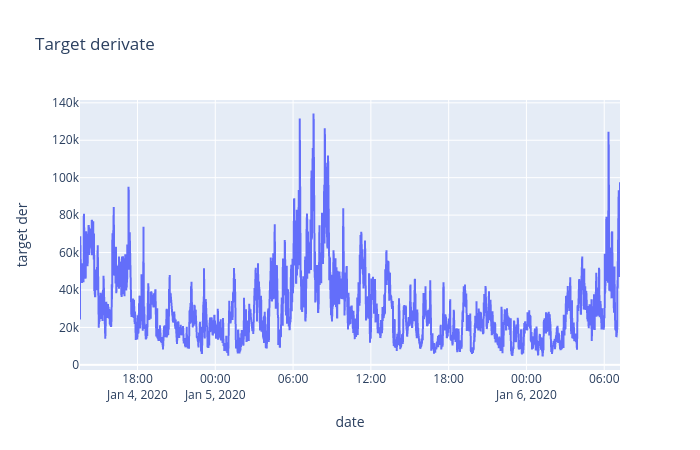
\includegraphics[width=\linewidth]{Figures/Y-J_before.png}
		\caption{Производная целевой переменной}\label{fig:yeo_before}
		\endminipage\hfill
		\minipage{0.49\textwidth}
		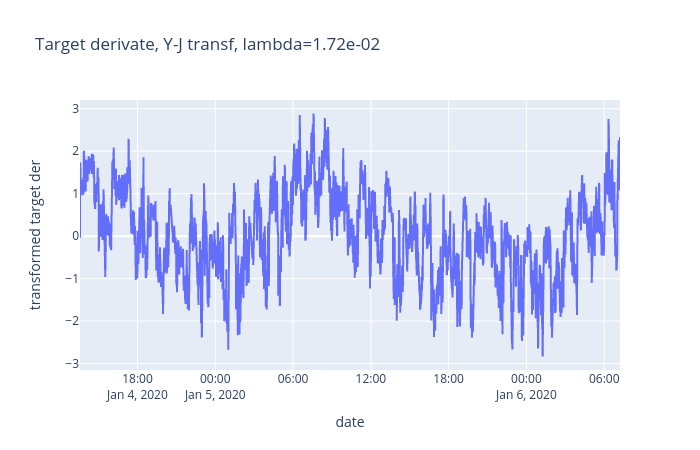
\includegraphics[width=\linewidth]{Figures/Y-J_after.png}
		\caption{Производная целевой переменной после масштабирования и преобразования Yeo-Johnson с $\lambda=1.72e-02$}\label{fig:yeo_after}
		\endminipage
	\end{figure}
	
	Это преобразование, действительно, стабилизирует дисперсию. Тем не менее стационарным этот ряд сделать не получилось. 

	Стоит отметить, что на самом деле это не сезонность.
	При более детальном рассмотрении, разница в ежедневных пиках загрузки может составлять и 15 минут и более. 
	Таким образом, если и есть подход, учитывающий сезонность, он должен быть достаточно рабастым.
	
	\section{Модель}
	\subsection{Описание классических моделей}
	Один из основных подходов к прогнозированию временных рядов - модели \texttt{SARMA(p, q) $\times$ (P, Q)}. Смысл аббревиатуры приведён ниже:
	\begin{enumerate}
		\item [S -] Модель учитывает сезонность длинны $S$
		\item [AR -] Модель учитывает признаки за $p$ предыдущих моментов времени.
		\item [MA -] Модель учитывает свои ошибки за $q$ предыдущих предсказаний
	\end{enumerate}
	Итоговую модель можно сформулировать следующим образом:
	\begin{align}
		y_t =\upvarepsilon_{t} + \phi_1y_{t-1} + \dots + \phi_py_{t-p} + \theta_1 \upvarepsilon_{t-1} + \dots + \theta_q \upvarepsilon_{t-q} + \nonumber \\
		\phi_S\cdot y_{t-S} + \dots + \phi_{PS} \cdot y_{t-SP} + \theta_S \cdot \upvarepsilon_{t-S} + \dots + \theta_{QS} \cdot \upvarepsilon_{t-QS} \nonumber
	\end{align}
	где $\upvarepsilon_{\tau} \sim \mathcal{N}(0, \sigma)$ - нормальный шум. Поскольку шум невозможно наблюдать, $\upvarepsilon_{\tau}$ вычисляется как ошибка предсказаний. Предсказания ряда строятся следующим образом:
	\begin{align}
	\hat{y}_t = \phi_1y_{t-1} + \dots + \phi_py_{t-p} + \theta_1 \upvarepsilon_{t-1} + \dots + \theta_q \upvarepsilon_{t-q} + \nonumber \\
	\phi_S\cdot y_{t-S} + \dots + \phi_{PS} \cdot y_{t-SP} + \theta_S \cdot \upvarepsilon_{t-S} + \dots + \theta_{QS} \cdot \upvarepsilon_{t-QS} \label{SARMA_est}
	\end{align}
	
	Обозначив коэффициенты $\phi_{\tau}$ и $\theta_{\tau}$ и имеющемся наборе данных можно составить серию предсказанных и известных значений, посчитать ошибку. 
	Как правило используют \texttt{MSE}, поскольку такая ошибка даёт несмещённые оценки. 
	Коэффициенты $\phi_{\tau}$ и $\theta_{\tau}$ находятся как решение оптимизационной задачи по минимизации ошибки.
	
	Стоит упомянуть, что $\hat{y}$ - оценка целевой переменной, а $y$ - признаковое описание системы, включающее лаг целевой переменной.
	
	Расширением является класс моделей \texttt{SARIMA(p, d, q) $\times$ (P, D, Q)} - ряд предварительно дифференцируется  \texttt{d} раз. 
	В данной работе построение начинается с \texttt{SARIMA, d = 1}. Впоследствии возможен перебор и этого гиперпараметра.
	
	Описание важных особенностей системы в данной работе приведено через поэтапное построение модели.

	\subsection{AR(p)}
	
	Строить \texttt{SARMA} - схожие модели мы будем используя линейную регрессию. 
	Предсказывать мы будем $y_t$, а в качестве признаков будем использовать не только значения $y_{t-i}$, как в \ref{SARMA_est}, но и другие метрики, которые наблюдает Acronis, и их значения в предыдущие моменты. 
	В итоге задача сводится к простой линейной регрессии.
	
	Для начала положим \texttt{p=1}. Как оказалось, рассмотрение даже такого небольшого класса позволит увидеть некоторые закономерности в данных. 
	Для начала сформируем выборки для теста и обучения. 
	Варьируя размер обучающей выборки построим график ошибки от размера обучающего набора данных. 
	Он представлен на рис.\ref{fig:test-train_mse}. 
	Оценкой качества модели считается \texttt{MAE}. 
	Внезапный скачок ошибки обусловлен единичным выбросом, детальней можно пронаблюдать эту ситуацию на рис.\ref{fig:outlier} и рис.\ref{fig:outlier_closer}.

	
	\begin{figure}[!htb]
		\minipage{0.49\textwidth}
		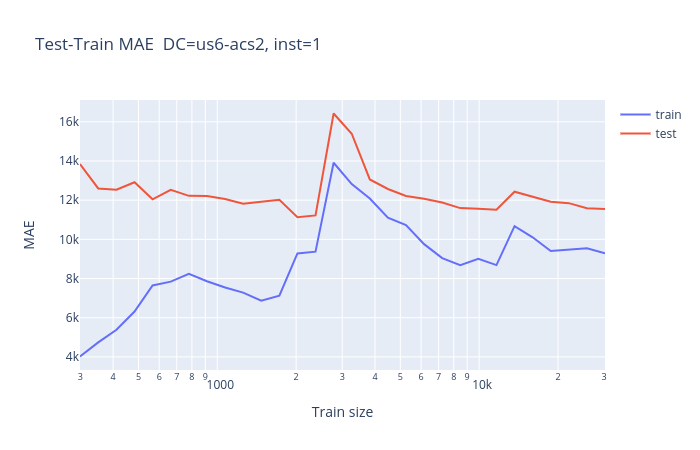
\includegraphics[width=\linewidth]{Figures/Test-Train_MSE.png}
		\caption{Зависимость ошибки на тестовой и обучающей выборке от размера обучения. В качестве ошибки для минимизации использовалось MSE. dc=us6-acs2, inst=23}\label{fig:test-train_mse}
		\endminipage\hfill
		\minipage{0.49\textwidth}
		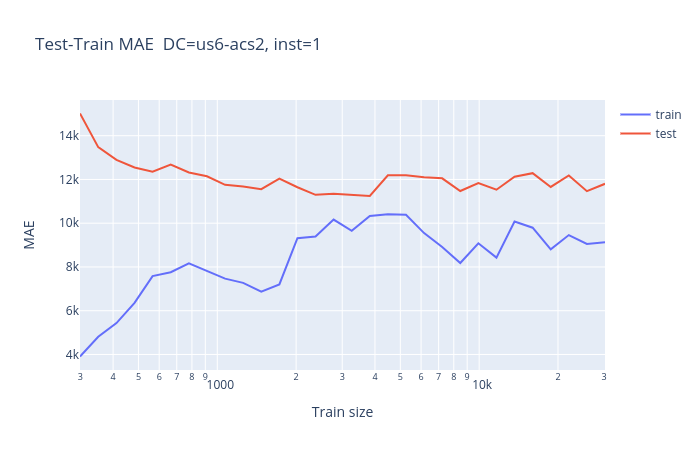
\includegraphics[width=\linewidth]{Figures/Test-Train_Hubert.png}
		\caption{Зависимость ошибки на тестовой и обучающей выборке от размера обучения. В качестве ошибки для минимизации использовался Hubert Loss. dc=us6-acs2, inst=1}\label{fig:test-train_hubert}
		\endminipage
	\end{figure}
	
	\begin{figure}[!htb]
		\minipage{0.49\textwidth}
		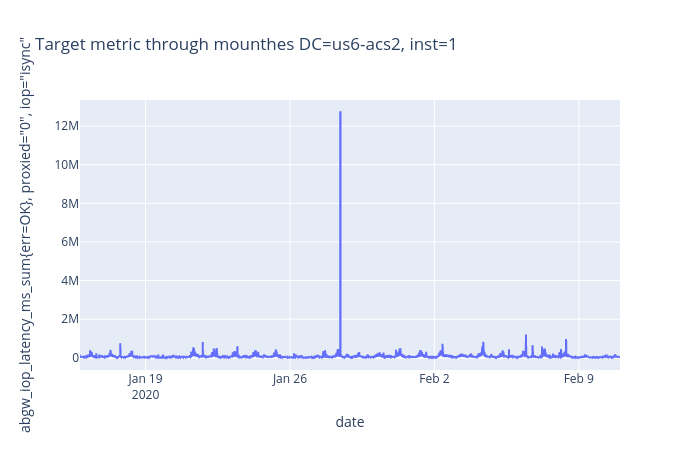
\includegraphics[width=\linewidth]{Figures/outlier.png}
		\caption{Единичный выброс, dc=us6-acs2, inst=23}\label{fig:outlier}
		\endminipage\hfill
		\minipage{0.49\textwidth}
		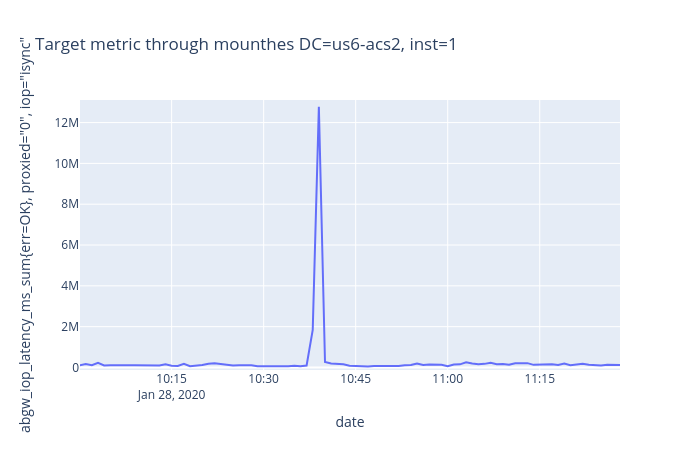
\includegraphics[width=\linewidth]{Figures/outlier_but_closer.png}
		\caption{Единичный выброс, увеличенный dc=us6-acs2, inst=1}\label{fig:outlier_closer}
		\endminipage
	\end{figure}
	
	Как видно на рис. \ref{fig:test-train_mse}, выброс портит не только ошибку на обучении, но и на отложенной выборке. Это показывает необходимость либо сменить метрику, либо удалить выбросы из обучающей выборки.
	В \ref{SARMA_est} нужны предыдущие значения и удаление одной точки приведёт к невозможности осуществить качественные расчёты для множества других. 
	Другой интересный подход к такой проблеме - использование не \texttt{MSE}, а \texttt{Hubert Loss}, что представляет из себя параболу, продолженную линейно после некоторого $\upvarepsilon$.
	Решение оптимизационной задачи в сформированном признаковом пространстве \texttt{X} в \ref{HubertOpt}, где $w$ - обобщённый вектор параметров $\phi$ и $\theta$, $alpha$ - коэффициент регуляризации.
	$y$ - целевая переменная.
	Параметр $\varepsilon=1.35$ устанавливается по умолчанию. 
	\begin{align}
	\min_{w, \sigma} {\sum_{i=1}^n\left(\sigma + H_{\epsilon}\left(\frac{X_{i}w - y_{i}}{\sigma}\right)\sigma\right) + \alpha {||w||_2}^2}\label{HubertOpt}\\
	H_{\upvarepsilon}(z) = 
	\begin{cases}
	z^2,  \quad\text{if }z \leq \upvarepsilon\\
	2\upvarepsilon|z| - \upvarepsilon^2, \ \text{otherwise}\
	\end{cases} \nonumber
	\end{align}
	
	Результат использования такой оптимизационной задачи можно видеть на рис.\ref{fig:test-train_hubert} Далее в работе коэффициенты для модели находятся решением \ref{HubertOpt}. Возвращаясь к размеру обучающей выборки, стоит отметить, что значимое уменьшение перестаёт наблюдаться при размере обучения около полутора дней. Скорость вычислений и представленный объём данных позволяют выбрать этот размер обучения равный трём дням.
	
	Следующим шагом логично поставить рассмотрения использования \texttt{p > 1}. 
	Качество модели в при подборе гиперпараметра, в этой работе, предлагается оценивать с помощью валидации. 
	Для временных рядов в процессе валидации не должно происходить тестирование в момент, предшествующий обучению. 
	Предложена следующая техника:
	\begin{enumerate}
		\item Зафиксировать размер обучения и тестирования
		\item Тестовую выборку выбрать как продолжение обучающей. 
		\item Обучить модель и протестировать. Оценивать качество при помощи \texttt{MAE}.
		\item Сдвинуть тестовую и обучающую выборку на минимум из размера обучения и теста.
	\end{enumerate}
	Результат такого перебора для \texttt{p=3} представлен на рис.\ref{fig:p-selection}.
	Имея $e_1$ ошибку при \texttt{p=1} и вычислив $e_2$ ошибку при другом \texttt{p} на графике отображёно $\frac{e_2 - e_1}{e_1}$.
	
	\begin{figure}[h]
		\centerline{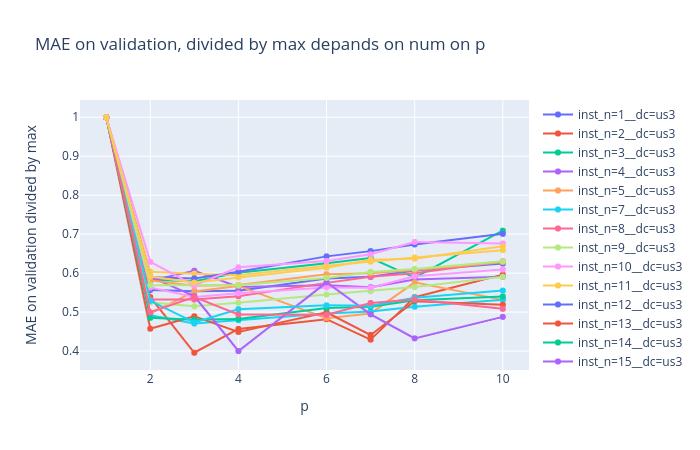
\epsfig{file=Figures/p-selection.png, scale=0.8}}
		\caption{Доля уменьшения MAE на валидации для us3}
		\label{fig:p-selection}
	\end{figure}
	Почти для всех интсансов характерно следующее поведение - резкое улучшение качества про добавлении одного лага.
	Все дальнейшие добавления не несут пользы, а лишь зашумляют модель.
	Выбор \texttt{p=2} позволяет допустить значимое увеличение ошибки и не допустить переобучения. 
	
	\subsection{Отбор метрик}
	После получения первого приближения качественной модели можно преступить к отбору метрик.
	Это позволит побороть переобучение в модели и, возможно, использовать больше лагов.	
	
	Основной подход предполагает определение универсального набора метрик для всех инстансов. Полная процедура следующая:
	\begin{enumerate}
		\item Для каждого инстанса с помощью Lasso регуляризатора отбирается число признаков. 
		Критерий выбора числа - отсутствие значимого увеличения точности при добавлении ещё одного признака.
		\item Выбор числа признаков универсально для всех инстансов. 
		Оказывается, что искомое число признаков практически совпадает.
		\item Для каждого инстанса строится модель на выбранных метриках.
		\item По полученным коэффициентам регрессии происходит отбор метрик - выбираются метрики с наибольшей по модулю границей разброса.
		Если $coeffs$ - это набор коэффициентов регрессии для выбранного признака, то сравниваются 
		$abs(coeffs.mean()) + coeffs.std()$ 
	\end{enumerate}

	\begin{figure}[!htb]
		\centerline{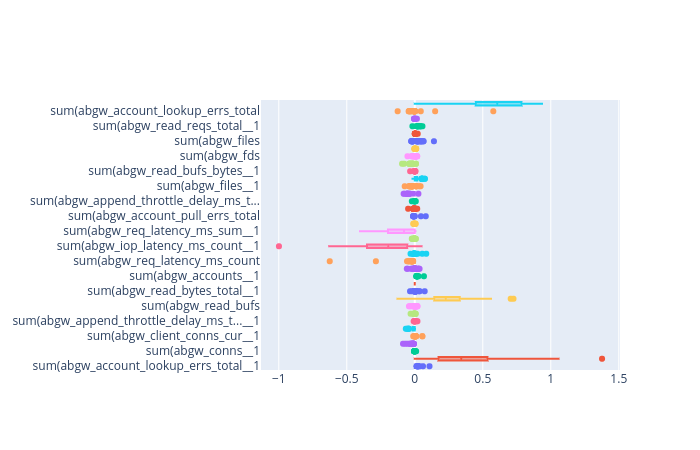
\epsfig{file=Figures/coeffs_boxplot.png, scale=0.8}}
		\caption{BoxPlot для коэффициентов регрессий}
		\label{fig:coeffs_boxplot}
	\end{figure}
	На рис.\ref{fig:coeffs_boxplot} представлен разброс метрик и легко можно выделить самые значимые.
	Тем не менее представленные результаты не совсем результат отбора. 
	Для начала коэффициенты получены при построении модели с Lasso регуляризатором и ошибкой MSE, в то время как предложено было использовать HubertLoss.
	Кроме того Lasso отбирала признаки, а не метрики.
	Для полной уверенности в результатах необходимо посмотреть как меняется точность модели при различном числе метрик.
	Результаты уменьшения ошибки представлены на рис.\ref{fig:mae_num_of_m}.
	
	\begin{figure}[!htb]
		\centerline{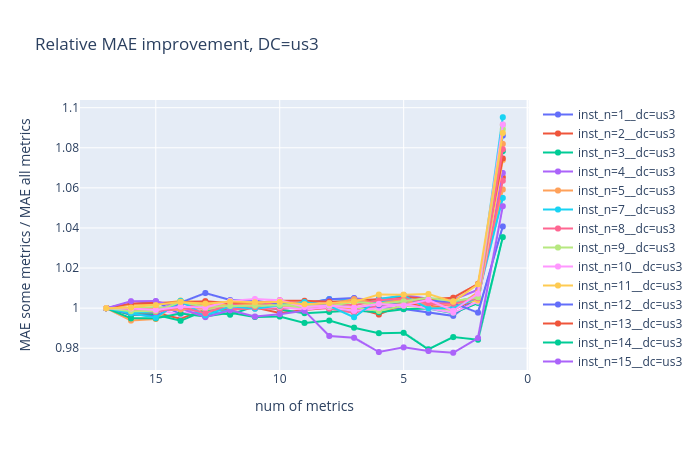
\epsfig{file=Figures/mae_nom_of_metrics.png, scale=0.7}}
		\caption{Результаты уменьшения ошибки для различного числа метрик на us3}
		\label{fig:mae_num_of_m}
	\end{figure}

	Видно, что изменение качество происходит совсем незначительное, поэтому имеет смысл оставить только лишь 4 метрики.
	
	Хотелось бы отметить, что принципиально важно провести отбор признаков до построения \texttt{ARMA} модели.
	Уменьшение размерности пространстве позволяет не сильно переопределить систему.
	При этом вместо не информативных признаков и их лагов в модели могут использоваться большие лаги информативных признаков и  лагов ошибок.

	\begin{figure}[!htb]
		\centerline{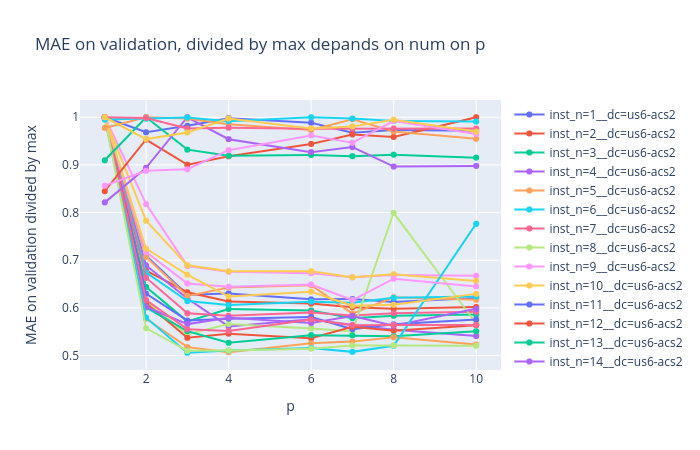
\epsfig{file=Figures/p_after_metric_selection.png, scale=0.7}}
		\caption{Уменьшение ошибки в зависимости от параметра \texttt{p} после отбора признаков}
		\label{fig:p_after_metric_selection}
	\end{figure}	
	
	
	\begin{figure}[!htb]
		\centerline{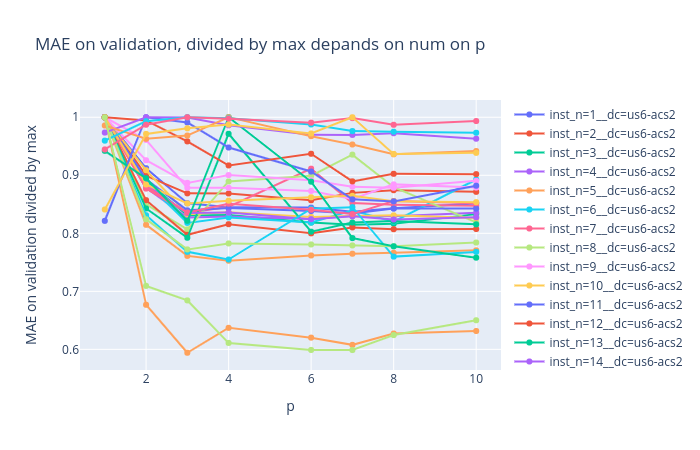
\epsfig{file=Figures/p_before_metric_selection.png, scale=0.7}}
		\caption{Уменьшение ошибки в зависимости от параметра \texttt{p} до отбора признаков}
		\label{fig:p_before_metric_selection}
	\end{figure}

	На рис.\ref{fig:p_after_metric_selection}, \ref{fig:p_before_metric_selection} можно наблюдать разницу влияния параметра \texttt{p} до и после отбора признаков.
	
	
	\subsection{ARMA(p, q)}
	В этой части предлагается провести исследование \texttt{ARMA(p,q)} \ref{ARMA_est} модели.
	\begin{align}
	\hat{y}_t = \phi_1y_{t-1} + \dots + \phi_py_{t-p} + \theta_1 \upvarepsilon_{t-1} + \dots + \theta_q \upvarepsilon_{t-q}\nonumber \\ \label{ARMA_est}
	\end{align}
	Важно обсудить оценку обучение модели и применение.
	
	При построении модели нужно учитывать шум $\upvarepsilon$ на предыдущих участках. Он не наблюдается, можно оценить построенной AR моделью на первом шаге, а затем несколько раз уточнить. Подобный подход, как самый наивные, описывается в \cite{lib_arma_est}. Количество уточняющих повторений обозначим за $k$.
	
	Ниже сформулирован подход к обучению модели ARMA:
	\begin{enumerate}
		\item Построить AR модель, с её помощью оценить коэффициенты для метрик их лагов.
		\item Оценить ошибку при помощи AR модели и добавить её и её лаги к признаковому описанию.
		\item Построить новую модель, учитывающую ошибку. Подсчитать ошибку и обновить её.
		\item Повторить предыдущий шаг $k_train$ раз.
	\end{enumerate}
	
	Ниже сформулирован подход к применению обученной модели ARMA:
	\begin{enumerate}
		\item К признаковому описанию добавить $q$ признаков, обозначающих ошибку. Их определить нулями.
		\item Построить регрессионную модель и оценить ошибку и её лаги.
		\item Построить новую модель, учитывающую ошибку. Подсчитать ошибку и обновить её.
		\item Повторить предыдущий шаг $k_test$ раз.
	\end{enumerate}
	
	Осуществить подбор $k_{test}$ и $k_{train}$ можно, проанализировав изменения коэффициентов модели и ошибки.

	\begin{figure}[!htb]
		\centerline{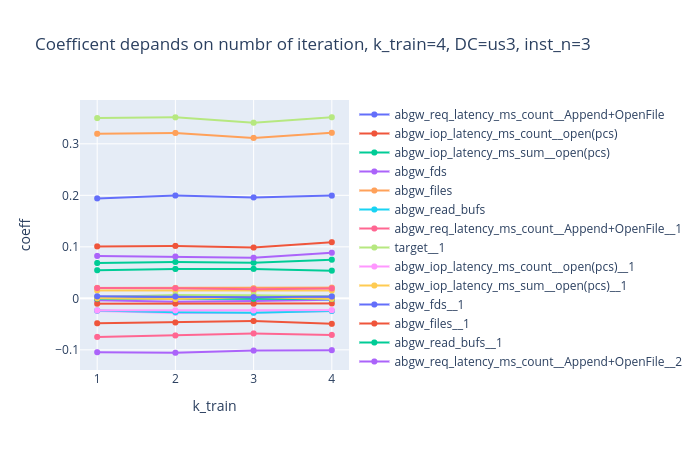
\epsfig{file=Figures/k_train_search.png, scale=0.6}}
		\caption{Зависимость коэффициентов регрессиии от числа итераций при построении ARMA}
		\label{fig:k_train_search}
	\end{figure}	
	
	\begin{figure}[!htb]
		\centerline{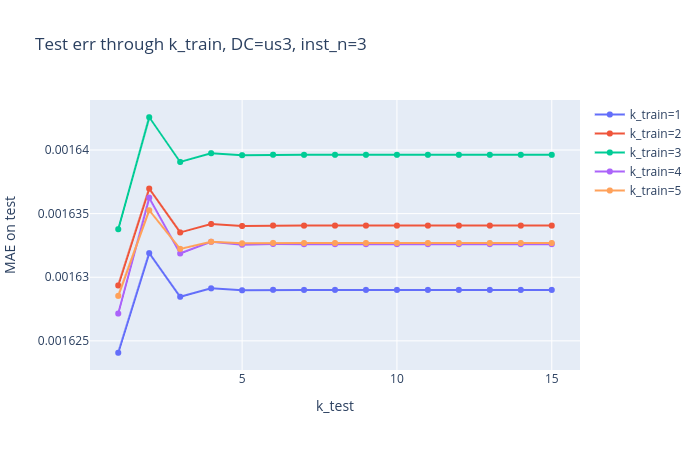
\epsfig{file=Figures/k_test_search.png, scale=0.6}}
		\caption{Зависимость точности от числа итераций ARMA при применении}
		\label{fig:k_test_search}
	\end{figure}	
	
	
	Такой подбор представлен на рис.\ref{fig:k_train_search}, \ref{fig:k_test_search}.
	Применение ARMA не требует большого числа итераций - хватит 4 для применения и 2 для прмиенения.
	Стоит отметить, что предложеные изменения не дают большого уеличения точности, поэтому следующим шагом предлагаю сравнить модель с подобранным \texttt{q, $k_{test}$, $k_{train}$} c первой моделью \texttt{AR}.
	
	\begin{figure}[!htb]
		\centerline{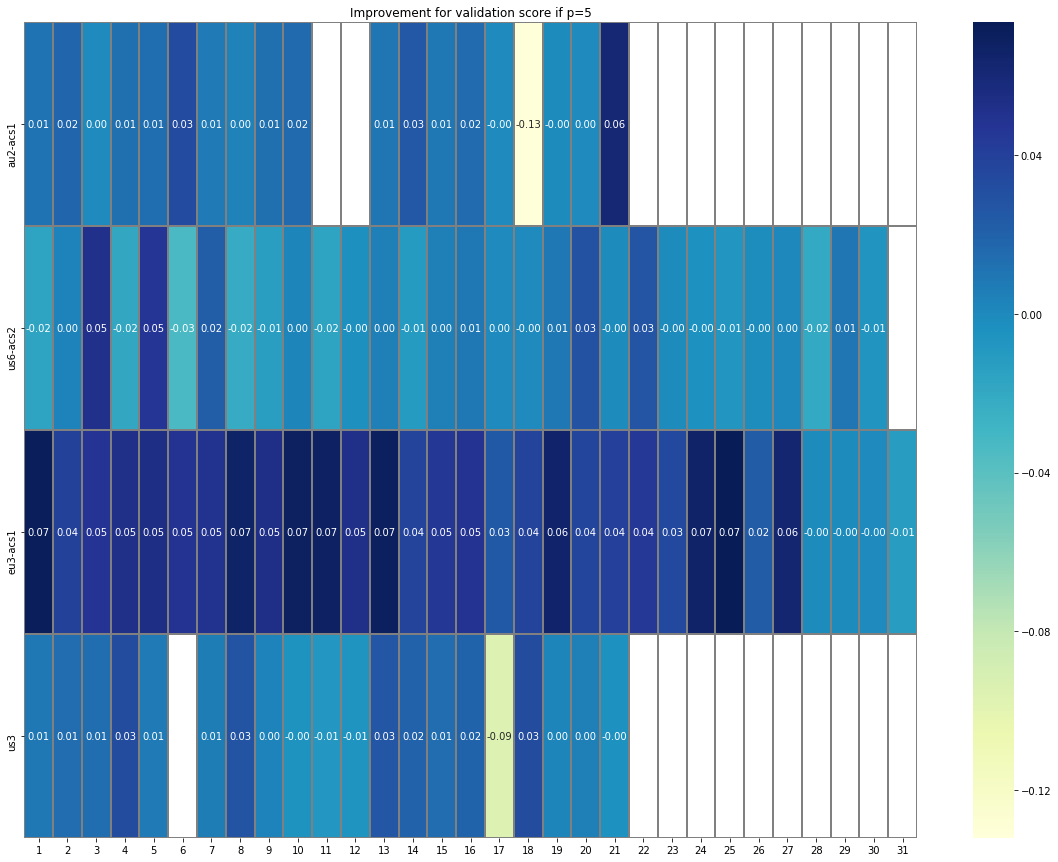
\epsfig{file=Figures/arma_vs_ar_hm.png, scale=0.5}}
		\caption{Относительное умнтшение MAE при испоьзованиие ARMA модели в сравенинии с AR для каждого инстанса}
		\label{fig:arma_vs_ar_hm}
	\end{figure}		
	
	\begin{figure}[!h]
		\centerline{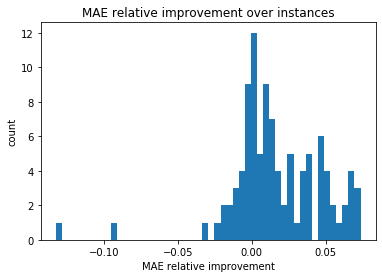
\epsfig{file=Figures/arma_vs_ar_hist.png, scale=1}}
		\caption{Относительное умнтшение MAE при испоьзованиие ARMA модели в сравенинии с AR}
		\label{fig:arma_vs_ar_hist}
	\end{figure}		
	
На рис. \ref{fig:arma_vs_ar_hm}, \ref{fig:arma_vs_ar_hist} представлено относительное уменьшение \texttt{MAE} на валидации при выборе \texttt{ARMA} модели. 
Таким образом, можно отметить, что значимого улучшения не наблюдается на большинсве инстансах, однако на некоторй группе оно есть значительное.
Поэтому имеется смысл в исспользовании \texttt{ARMA} модели.	
	
На текущем этапе исследования модели также имеется возможность рассматривать модель при трёх важных гипрепараметрах: количество признаков, \texttt{p}, \texttt{q}.
	
	\subsection{Корректность модели}
После построения предсказательной модели овзникает вопрос о том, корректна ли эта модель. Для этого нужно проверить слудеющие характеристики: распределние ошибки и её гетероскедастичность. Также нужно рассмотреть стационарность временного ряда ошибки. 
Для начала обсудим гетероскичность - независимость ошибки от целевой переменной.
Самоё простое что можно сделать - посмотреть на ошибку в зависимости от целевой переменной.
Стоит отметить наличие двух принципиально рзных случаев - \texttt{AR(p$\neq0$)} и \texttt{AR(0)}.

	\begin{figure}[!htb]
		\minipage{0.49\textwidth}
		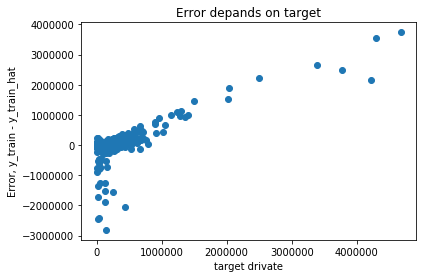
\includegraphics[width=\linewidth]{Figures/heter_p_neq_0.png}
		\caption{Зависимость ошибки от целевой переменной в модели с учётом лагов}\label{fig:heter_p_neq_0}
		\endminipage\hfill
		\minipage{0.49\textwidth}
		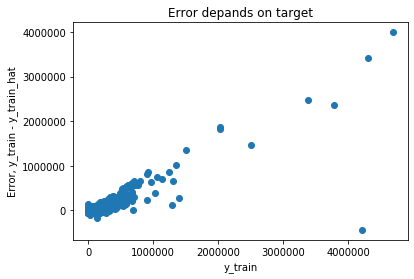
\includegraphics[width=\linewidth]{Figures/heter_p_eq_0.png}
		\caption{Зависимость ошибки от целевой переменной в модели с без учёта лагов}\label{fig:heter_p_eq_0}
		\endminipage
	\end{figure}	

Интересно, что на рис. \ref{fig:heter_p_neq_0} есть участок, соответствующий отрицательным ошибкам на участках с низкими значениями целевой переменной.
На рис.\ref{fig:heter_p_eq_0} такого участка не наблюдается.
Это может быть обусловлено учётом лагов.
Наличие выброса, кроме большой ошибки в текущий момент повлечёт ошибку при учёте выброса, как лага. 

Тем не менее признак некачественной модели - зависимость ошибки от цлелевой переменной.
Одной из причин такого поведения может быть неверное масштабирование, ведь при маштабировании по формуле (\ref{MinMax_sc}) основная масса значений оказывается около нуля из-за наличия выбросов. 
Таки образом ошибка \texttt{Hubert} почти не настраивается на большие значения ошибок и целевой переменной и при модель получается в некоторм смысле смещённой.
Это происходит изза того, что распределение целевой переменной не обладает хоть какой-нибудь симметрией.
Один из сопсобов расрпеделить влеичины более равномерно - исопльзовать преобразование Yeo-Johnson (\ref{Yeo-Joh}).

	\begin{figure}[!htb]
		\minipage{0.49\textwidth}
		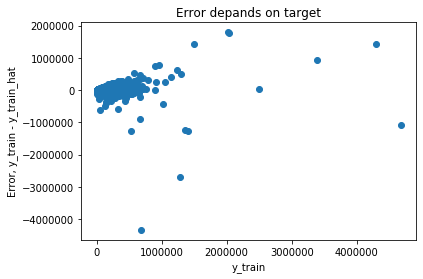
\includegraphics[width=\linewidth]{Figures/heter_pt.png}
		\caption{Зависимость ошибки от целевой переменной в модели с учётом лагов и преобразование (\ref{Yeo-Joh})}\label{fig:heter_pt}
		\endminipage\hfill
		\minipage{0.49\textwidth}
		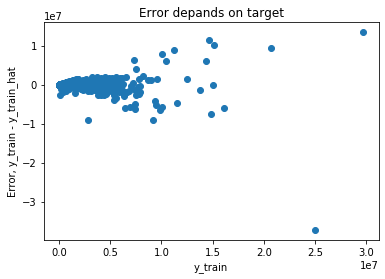
\includegraphics[width=\linewidth]{Figures/heter_sum.png}
		\caption{Зависимость ошибки от целевой переменной в модели с учётом лагов, усреднённая за 5 мин}\label{fig:heter_sum}
		\endminipage
	\end{figure}	
	
На рис.\ref{fig:heter_pt} видно, что после применения другого способа масштабирования ошибка стала меньше зависеть от цлеелвой переменной.
Тем не менее заметна небольшая тенденция к возрастанию. Пока что такое поведение можно объяснить высокой дискретностью данных и резкимими перепадами. Если же избавиться от резких перепадов, нарпример усреднением за 5 минут, то такое возрастанние исчезает, как на рис. \ref{fig:heter_sum}. Кроме того стоит отметить, что разброс ошибки сильно уменьшился в особые, систематически более загруженные периоды времени.


\section{Заключение}

В представленной работе произведё качественное и количественное исследование класса мделей \texttt{ARMA} для продукта Acronis Storage.
Результатом исследования стало:
\begin{itemize}
\item Схемы выбора важных для описания системы метрик
\item Линейная модель, предназначение котрой - быть инструментом для определения аномального поведения.
\end{itemize}

В ходе исследования были применены:
\begin{itemize}
\item Различные подходы к масштабированию
\item \texttt{LASSO} регуляризатор для отбора признаков
\item Различные функции ошибки
\end{itemize}

Ни сезонностью, ни преобразовниями Yeo-Johnson добиться стационарности ряда про критерию \texttt{KPSS} не удалось.
Также не удалось добиться достаточного уровня значимости для принятия гипотезы о стационарности ошибки.
Тем не менее гистограмммы и графики ошибки от времени показывают воодушевляющие результаты.
	
	\begin{thebibliography}{228}
	
		\bibitem{lib_prometheus} 
		\emph{Prometheus - an open-source systems monitoring and alerting toolkit.} \\
		URL: https://prometheus.io/.
		
		\bibitem{lib_large_samples} 
		\emph{How do we know which test to apply for testing normality} \\
		URL: https://www.researchgate.net
		
		\bibitem{lib_sklearn_transformer_outliers} 
		\emph{Sk Learn - Compare the effect of different scalers on data with outliers} \\
		URL: https://scikit-learn.org	
		
		\bibitem{lib_arma_est}
		\emph{Lesson 12,  Estimation of the parameters of an ARMA model} \\
		URL: http://www.phdeconomics.sssup.it
		
		\end{thebibliography}
			
\end{document}
